
\subsection{Inference of Dictionary}
A well learned Dictionary is the key for sparse coding method because if the dictionary is not well learned, the sparse coding step will have trouble in properly reconstructing the input data.\\
Here we expose only a few methods which aim to well learn a dictionary: The first two algorithms learn the dictionary D using the whole training set, unlike the third one wich learn D by using an iterative batch procedure. The last method is a well-known algorithm based on singular value decomposition.

\subsubsection{Algorithm 1: Gradient Descent }

\begin{figure}[h]
 \centering
 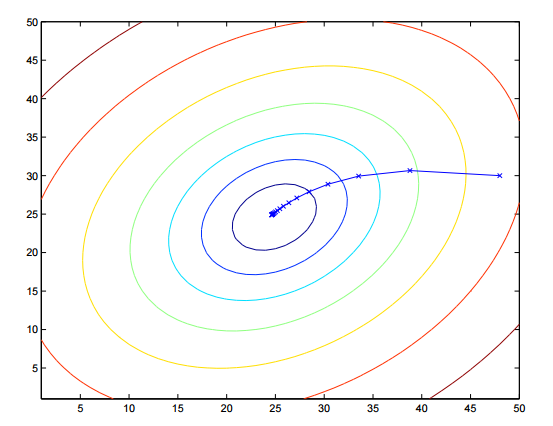
\includegraphics[scale=0.3]{ellipses.png}
 % ellipses.png: 553x426 px, 72dpi, 19.51x15.03 cm, bb=0 0 553 426
 \caption{Example of gradient descent}
 \label{fig:gradientDescent}
\end{figure}

%\paragraph{Algorithm 1: A gradient descent method}
To minimize Sparse Coding and dictionary learning's cost function we must use all our knowledge of mathematical optimization. There are many optimizations algorithm that can find an approximation which minimizes Sparse Coding and dictionary learning's cost function. Most famous one is the gradient descent, its simplicity of implementation and its results are no longer to be proved. It becomes an indispensable tool for Machine learning scientist.\\
The main idea is to find the local minimum of a cost function iteratively. At each step, the parameters are updating proportionally (this is step size, controlled by a learning rate $\lambda$) in the opposite direction of the gradient of the objective function (see figure \ref{fig:gradientDescent}).\\
As a reminder, our objective function is:
\begin{center}
 $\min\limits_{D} \frac{1}{n} \sum_{i=1}^{n}  \min\limits_{\gamma} \frac{1}{2} \| x_i - D \hspace{3px} \gamma \|_2^2 + \lambda \|\gamma_i \|_1$\\
\end{center}
In the dictionary learning step we assume that $\gamma$ is fixed and D variable. We can simplify our problem without all terms which do not depend on the dictionary D, let's define a function $f$ such that:
\begin{center}
 $f(D) = \min\limits_{D} \frac{1}{n} \sum_{i=1}^{n}\frac{1}{2} \| x_i- D \hspace{3px} \gamma_i \|_2^2 $\\
\end{center}
Then we can compute the gradient of $f(D)$:

\begin{center}
 $\bigtriangledown f(D) = \frac{1}{n} \sum_{i=1}^n (x_i -D \gamma_i)\gamma_i^{\intercal}$
\end{center}

\begin{algorithm}
\caption{Dictionary Learning: Gradient descent}
 \begin{algorithmic}
  \REQUIRE x, $\gamma$, $\alpha$
  \WHILE{D not converged}
        \STATE \textit{// Perform gradient descent update of D}
        \STATE $D = D - \alpha * (X-D\gamma)*\gamma^{\intercal}$
        \STATE \textit{// Renormalize columns of D}
        \FOR{ each column j of D}
            \STATE $D[:,j] = \frac{D[:,j]}{\|D[:,j]\|}$
        \ENDFOR
  \ENDWHILE
  \RETURN D
 \end{algorithmic}
\end{algorithm}

%\begin{lstlisting}[language=Python,frame=single]
%while D not_converged:
%    # Perform gradient update of D
%    D = D - alpha * (1/T)* sum((x - D h)* tranpose(h))
%    # Renormalize the columns of D
%    for each column D[:,j]:
%        D[:,j] = (D[:,j] / norm(D[:,j]))
%
%return D
%\end{lstlisting}

\subsubsection{Algorithm 2: Block-coordinate descent}

\begin{figure}[h]
 \centering
 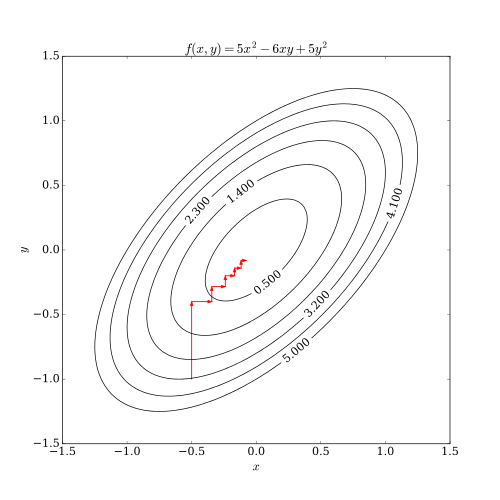
\includegraphics[scale=0.4]{Coordinate_descent.png}
 % Coordinate_descent.svg.png: 500x500 px, 72dpi, 17.64x17.64 cm, bb=0 0 500 500
 \caption{Example of Block-Coordinate descent}
 \label{fig:BlockCoordDescent}
\end{figure}

%We must minimize:
%\begin{center}
 %$\min\limits_{D} \frac{1}{T} \sum_{t=1}^{T}  \min\limits_{\gamma} \frac{1}%{2} \| x^{(t)} - D \hspace{3px} \gamma \|_2^2 $\\
%\end{center}
To avoid the learning rate there are other algorithms that can be applied instead of gradient descent. One of them is called Block-coordinate descent. The idea is to find the minimum of our objective's function for each direction in a cycle, in this case, a direction is a column of $D_{., j}$ (see figure \ref{fig:BlockCoordDescent}). Firstly, we have to set the gradient of $D_{., j}$ to zero.\\
\begin{center}
 $ \frac{1}{n}\sum_{i=1}^{n} (x_i - D \gamma_i)$ $\gamma_{[i,j]} = 0$\\ \vspace{0.4cm}
 We separe $D_{.,j}$ from the rest of D:\\
 $\iff 0 = \frac{1}{n}\sum_{i=1}^{n} (x_i - (\sum_{l \neq j}D_{.,l}$ $\gamma_{[i,l]}$ $ )$  $ - (D_{.,j}$ $\gamma_{[i,j]})$ ) $ \gamma_{[i,j]}$\\ \vspace{0.4cm}
 Our aim is to find the value of $D_{.,j}$, we must isolate $D_{.,j}$ :\\
 $\iff 0 = \frac{1}{n} \sum_{i=1}^{n}(x_i \gamma_{[i,j]} - (\sum_{l \neq j}D_{.,l}$ $\gamma_{[i,l]}$ $\gamma_{[i,j]} )$  $ - (D_{.,j}$ $\gamma^2_{[i,j]}))$\\ \vspace{0.2cm}
  $\iff 0 = (\sum_{i=1}^{n}(x_i \gamma_{[i,j]} - (\sum_{l \neq j}D_{.,l}$ $\gamma_{[i,l]}$ $\gamma_{[i,j]} )$  $) - ( \sum_{i=1}^{n}( D_{.,j}$ $\gamma_{[i,j]}^2)))$\\ \vspace{0.2cm}
  
  $ \iff \sum_{i=1}^{n}( D_{.,j}$ $\gamma^2_{[i,j]}) = \sum_{i=1}^{n}(x_i \gamma_{[i,j]} - (\sum_{l \neq j}D_{.,l}$ $\gamma_{[i,l]}$ $\gamma_{[i,j]} )$  $) $\\  \vspace{0.2cm}
  
  $\iff D_{.,j}  \sum_{i=1}^{n} \gamma^2_{[i,j]} = \sum_{i=1}^{n}(x_i \gamma_{[i,j]} - (\sum_{l \neq j}D_{.,l}$ $\gamma_{[i,l]}$ $\gamma_{[i,j]} )$  $) $\\ \vspace{0.2cm}
  
$\iff D_{.,j}  =\frac{1}{ \sum_{i=1}^{n} \gamma^2_{[i,j]}}\sum_{i=1}^{n}(x_i \gamma_{[i,j]} - (\sum_{l \neq j}D_{.,l}$ $\gamma_{[i,l]}$ $\gamma_{[i,j]})$  $) $\\ \vspace{0.2cm}

$\iff D_{.,j}  =\underbrace{\frac{1}{ \sum_{i=1}^{n} \gamma^2_{[i,j]}}}_{A_{j, j}} \underbrace{\sum_{i=1}^{n}(x_i \gamma_{[i,j]})}_{B_{., j}}  - \sum_{l \neq j}D_{., l}($ $\underbrace{\sum_{i=1}^{n} \gamma_{[i,l]} \alpha_{[i,j]} ) }_{A_{i,j}}$\\ \vspace{0.2cm}
$D_{., j} = \frac{1}{A_{j, j}}(B_{., j} - D A_{., j} + D_{., j}A_{j, j})$
\end{center}  

\begin{algorithm}
 \caption{Dictionary Learning: Block-coordinate descent}
 \begin{algorithmic}
    \REQUIRE X, $\gamma$
    \WHILE{ D not converged}
        \FOR{ each column j of D}
            \STATE \textit{// For each column D[:,j] perform update}
            \STATE $D[:,j] = \frac{1}{A[j,j]}  (B[:,j] - D  A[:,j] + D[:,j]  A[j,j])$
            \STATE \textit{// Normalization}
            \STATE $D[:,j] = \frac{D[:,j]}{\|D[:,j]\|}$
        \ENDFOR
    \ENDWHILE
    \RETURN D
 \end{algorithmic}

\end{algorithm}

%\begin{lstlisting}[language=Python,frame=single]
%while D not_converged:
%    # For each column D[:,j] perform updates
%    for each column D[:,j]:
%        D[:,j] = (1/A[j, j])*(B[:, j] - D A[:, j] + D[:, j] A[j, j])
%        # Normalization
%        D[:,j] = D[:,j]/norm(D[:,j])
%
%return D
%\end{lstlisting}

\subsubsection{Algorithm 3:  Online learning algorithm}
Today with the improvement of datasets size, it is impossible to train the dictionary over the entire dataset. To address this problem, machine learning scientist uses the online learning methods. Instead of learning on the entire dataset its update the model for each sample. In our case, we will update the dictionary after visiting each $x_i$. Mairal proposed  \cite{Mairal:2009:ODL:1553374.1553463} this online approach for the dictionary learning :
%\begin{itemize}
 %\item[$\bullet$]  Perform inference of $\gamma_i$ after visiting each $x_i$
% \item[$\bullet$]  Update running of the quantities required to update D: 
%        \begin{itemize}
%         \item B = $\beta B + (1 - \beta) x^{(t)}\gamma_i^T$
%         \item A = $\beta A + (1 - \beta)\gamma_i \gamma_i^T$
%        \end{itemize}
%\item[$\bullet$] Use current value of D as " warm start" to block-%coordinate descent (warm start $\iff$ With the previous value of D)
%\end{itemize}
%With $\beta$ a constant value use like a learning rate.

\begin{algorithm}
 \caption{Dictionary Learning: Online learning algorithm}
 \begin{algorithmic}
  \REQUIRE X, $\alpha$ (learning rate), T (number of iterations)
  \STATE $A = 0$, $B = 0$ (reset the ``past information"`)
  \STATE Initialize $D$ randomly (not to 0)
  \FOR{$t = 1$ to T}
    \STATE Infer code $\gamma$ from X
    \STATE $A = A + \gamma \gamma^{\intercal}$
    \STATE $B = B + X \gamma^{\intercal}$
    \FOR{$i = 1$ to n}
        \FOR{ each column j of D}
            \STATE $ D[:,j] = \frac{1}{A[j,j]}*(B[:,j] - D A[:,j] + D[:,j] A[j,j])$
            \STATE \textit{// Normalization}
            \STATE $D[:,j] = \frac{D[:,j]}{\|D[:,j]\|} $
        \ENDFOR
    \ENDFOR
  \ENDFOR
  \RETURN D
 \end{algorithmic}
\end{algorithm}


%\begin{lstlisting}[language=Python,frame=single]
%Initialize D # Not to 0 ! (To respect the constraint we define before)
%while D not_converged:
%    for each x:
%        Infer code h
%        #Update dictionary
%        A = A +  h * transpose(h)
%        B = B + x * transpose(h)
%        #Batch upgrade
%        #A = beta * A + ( 1 - beta ) * h * transpose(h)
%        #B = beta * B + ( 1 - beta ) * x * transpose(h)
%        while D not_converged:
%            for each column D[:,j]:
%                 D[:,j] = (1/A[j,j])*(B[:,j] - D A[:,j] + D[:,j] A[j,j])
%                # Normalization
%                D[:,j] = D[:,j]/norm(D[:,j]) 
%\end{lstlisting}
\paragraph{Optimizing the Algorithm}
In practice, it's possible to improve the convergence speed of this algorithm by using a Mini-batch extension: By drawing $\eta > 1 $ signals at each iteration instead of a single one. Thus we have:
\begin{center}
  \[    \left\{
                \begin{array}{ll}
                  A_t  = \beta A_{t-1} + \sum_{i=1}^{\eta} \alpha_{t,i}\alpha_{t,i}^{T}\\
                  B_t = \beta B_{t-1} + \sum_{i=1}^{\eta}x\alpha_{t,i}^{T}\\
                \end{array}
              \right.
  \]
\end{center}

With $\beta = \frac{\theta + 1 - \eta}{\theta +1}$, where $\theta = t \eta$ if $ t < \eta$ and $\eta^2 + t - \eta$ if $t \geq \eta$.


\subsubsection{Algorithm 4: K-SVD}
K-SVD is an algorithm proposed by Aharon, Elad, and Bruckstein \cite{1710377} that generalizes the K-mean clustering algorithm via a singular value decomposition (SVD) approach:

\begin{algorithm}
 \caption{K-SVD algorithm}
 \begin{algorithmic}
  \REQUIRE X
  \STATE Initialize D randomly
  \STATE  Ifer code $\gamma$ from X
   \FOR{ each column j of D}
    \STATE $GammaActive = \emptyset $
    \STATE $ActiveSet = \emptyset$
    \STATE $ErrorActiveSet = \emptyset$
    \FOR{i=1 to n}
        \IF{$\gamma_{[i,j]} \neq 0$}
            \STATE $GammaActive = GammaActive \bigcup gamma_{[i,j]}$
            \STATE $ActiveSet = ActiveSet \bigcup X_i$
            \STATE $temp = X_i$
            \FOR{ each $l$ such that $\gamma_{i,l} \neq 0$ and $l \neq j$}
                \STATE $temp = temp - D[:,l] $
            \ENDFOR
            \STATE $ErrorActiveSet = ErrorActiveSet \bigcup temp$
        \ENDIF
    \ENDFOR
    \STATE $D[:,j] = $ $\underset{D[:,j]}{\min}$ $\|ErrorActiveSet - D[:,j]*GammaActive)\|^2_2$   $
    \hspace{0.5cm}\Rightarrow$ This can be done by using SVD. 
  \ENDFOR
  \RETURN D
 \end{algorithmic}

\end{algorithm}
